\documentclass[11pt]{article}
\usepackage{fullpage,amsmath,amsfonts,mathpazo,microtype,nicefrac,graphicx}

% Set-up for hypertext references
\usepackage{hyperref,color,textcomp}
\definecolor{webgreen}{rgb}{0,.35,0}
\definecolor{webbrown}{rgb}{.6,0,0}
\definecolor{RoyalBlue}{rgb}{0,0,0.9}
\definecolor{purp}{rgb}{0.6,0.3,0.9}
\hypersetup{
   colorlinks=true, linktocpage=true, pdfstartpage=3, pdfstartview=FitV,
   breaklinks=true, pdfpagemode=UseNone, pageanchor=true, pdfpagemode=UseOutlines,
   plainpages=false, bookmarksnumbered, bookmarksopen=true, bookmarksopenlevel=1,
   hypertexnames=true, pdfhighlight=/O,
   urlcolor=webbrown, linkcolor=RoyalBlue, citecolor=webgreen,
   pdfauthor={Chris H. Rycroft},
   pdfsubject={Harvard AM205 (Fall 2014)},
   pdfkeywords={},
   pdfcreator={pdfLaTeX},
   pdfproducer={LaTeX with hyperref}
}
\hypersetup{pdftitle={AM205: Assignment 4}}

% Macro definitions
\newcommand{\N}{\mathbb{N}}
\newcommand{\Z}{\mathbb{Z}}
\newcommand{\Q}{\mathbb{Q}}
\newcommand{\R}{\mathbb{R}}
\newcommand{\C}{\mathbb{C}}
\newcommand{\B}{\mathbb{B}}
\newcommand{\p}{\partial}
\newcommand{\Trans}{\mathsf{T}}
\renewcommand{\vec}[1]{\mathbf{#1}}
\newcommand{\vx}{\vec{x}}
\newcommand{\vb}{\vec{b}}

\DeclareMathOperator{\rank}{rank}

\begin{document}
\section*{AM205: Assignment 4 (due 5~PM, November 7)}
\noindent \textit{For this assignment, first complete problems 1 and 2, and then
complete \textbf{either} problem 3 (on numerical PDEs) or problem 4 (on
optimization). If you submit answers for both problems 3 and 4, the maximum
score from the two will be taken when calculating your grade.}

\vspace{0.5em}
\noindent \textit{Program files: A number of program and data files for this
homework can be downloaded as a single ZIP file from the course website.}
\begin{enumerate}
  \item {\bf Convergence and stability of a numerical scheme.} Consider the
    numerical scheme
    \begin{equation}
      \frac{U_j^{n+1} - 2U_j^n + U_j^{n-1}}{\Delta t^2} - c^2 \frac{U_{j+1}^n - 2U_j^n + U_{j-1}^n}{\Delta x^2} = 0
      \label{eq:1dwave}
    \end{equation}
    to solve the one-dimensional wave equation $u_{tt} - c^2 u_{xx}=0$. Here,
    $c\in \R$ and $U_j^n$ is the numerical approximation of $u( j\Delta
    x,n\Delta t)$.
    \begin{enumerate}
      \item Show that the numerical scheme in Eq.~\ref{eq:1dwave} is second-order
	accurate.
      \item Use Fourier stability analysis, by subsituting in the ansatz \smash{$U_j^n
	= \lambda(k)^n e^{ijk\Delta x}$}, to show that the numerical scheme is
	stable. Because the wave equation is second-order in time, you will get
	two solutions $\lambda(k)$ for each $k$, and both must have magnitude
	less than or equal to 1 for stability.
    \end{enumerate}
  \item \textbf{Totally rocking out in Pierce Hall.} The image below shows a
    map of the third floor of Pierce Hall. All the doors are open, apart from
    those to the main stairwells and the passageway to Maxwell--Dworkin.
    \setlength{\unitlength}{0.9bp}
    \begin{center}
      \begin{picture}(400,200)
	\put(0,0){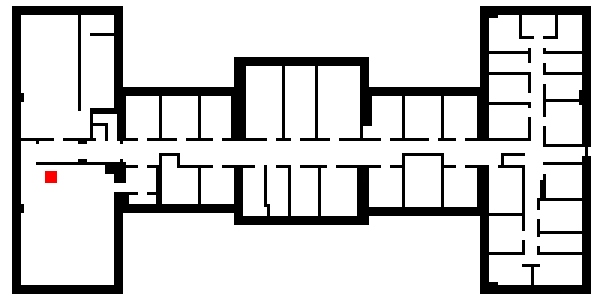
\includegraphics[width=400\unitlength]{am205_hw4_files/orig_image/pierce_large}}
	\put(40,78){\textcolor{red}{$S$}}
	\put(143,122){\textcolor{blue}{C}}
	\put(225,61){\textcolor{blue}{M}}
	\put(333,175){\textcolor{blue}{B}}
	\put(111,74){\scriptsize\textcolor{purp}{Stair}}
	\put(273,74){\scriptsize\textcolor{purp}{Stair}}
      \end{picture}
    \end{center}
    A text file \texttt{pierce.txt} is provided that encodes this map as a $100
    \times 200$ matrix using 1 for walls and 0 for empty space. Use the
    convention that $(j,k)=(0,0)$ is the top left of the matrix and
    $(j,k)=(99,199)$ is bottom right of the matrix. The grid spacing is
    $h=36.6\text{~cm}$.

    A group of students hold an event in Pierce 301, the large room in the
    bottom left of the map. They set up a loudspeaker shown in red, covering
    the region $S$ over gridpoints $(j,k)$ for $57\le j \le 60, 15\le k \le
    18$. When testing the speaker, they drive it with a $50\text{~Hz}$ sine
    wave,\footnote{The typical human auditory range is from $20\text{~Hz}$ to
    $20\text{~kHz}$, so this sound is at the lower end of what is audible.}
    creating sound pressure waves that travel throughout the building,
    disturbing the occupants. The pressure field $p(x,y,t)$ satisfies the wave
    equation
    \begin{equation}
      \frac{\p^2 p}{\p t^2} - c^2 \nabla^2 p =0, \label{eq:spde}
    \end{equation}
    where $c=3.43\times 10^4\text{~cm~s}^{-1}$ is the speed of sound. At $t=0$
    when the speaker is switched on, the pressure satisfies the initial
    conditions $p(x,y,t)=p_t(x,y,t)=0$. At each wall, the pressure satisfies
    the boundary condition
    \begin{equation}
      \vec{n} \cdot \nabla p = 0,\label{eq:pbc} 
    \end{equation}
    where $\vec{n}$ is a unit vector normal to the wall. In the region $S$
    the pressure is driven to satisfy
    \begin{equation}
      p(x,y,t)= f(t) = p_0 \sin \omega t, \label{eq:force}
    \end{equation}
    where the angular frequency is $\omega = 100\pi \text{~s}^{-1}$ and the
    pressure constant\footnote{This pressure is similar to what you might get
    at a rock concert.} is $p_0 = 10\text{~Pa}$.
    \begin{enumerate}
      \item Write a program to solve for the pressure field inside the
	building, using the two-dimensional discretization
	\begin{equation}
	  \frac{P_{j,k}^{n+1} - 2P_{j,k}^n + P_{j,k}^{n-1}}{\Delta t^2} - c^2 \frac{P_{j+1,k}^n + P_{j,k+1}^n - 4P_{j,k}^n + P_{j-1,k}^n+P_{j,k-1}^n}{h^2} = 0. \label{eq:2dwavefd}
	\end{equation}
	where \smash{$P_{j,k}^n$} is the numerical approximation of $p(jh,kh,n\Delta
	t)$. Use a timestep of \smash{$\Delta t = \frac{h}{2c}$} or smaller. As
	initial conditions, use
	\begin{equation}
	  P_{j,k}^0=0, \qquad P_{j,k}^1 = \left\{
	  \begin{array}{ll}
	    f(\Delta t) & \qquad \text{if $(j,k)\in S$,} \\
	    0 & \qquad \text{otherwise.}
	  \end{array}
	  \right.
	\end{equation}
	To account for the boundary condition in Eq.~\ref{eq:pbc}, use the
	ghost node approach: when considering a point $(j,k)$ in
	Eq.~\ref{eq:2dwavefd} that references an orthogonal neighbor $(j^*,k^*)$
	that is a wall, treat \smash{$P_{j^*,k^*}^n$} as equal to \smash{$P_{j,k}^n$}.
	As an example of this, suppose that at a particular $(j,k)$, the points
	$(j,k-1)$ and $(j+1,k)$ are within walls. Then, after taking into
	account the boundary conditions, the appropriate finite-difference
	relation is
	\begin{equation}
	  \frac{P_{j,k}^{n+1} - 2P_{j,k}^n + P_{j,k}^{n-1}}{\Delta t^2} - c^2 \frac{P_{j,k+1}^n - 2P_{j,k}^n + P_{j-1,k}^n}{h^2} = 0. \label{eq:2dwaverest}
	\end{equation}
	due to cancellation of some terms. To account for the condition in
	Eq.~\ref{eq:force}, enforce throughout the computation that
	\smash{$P_{j,k}^n = f(n\Delta t)$} for $(j,k)\in S$.
      \item Make two-dimensional plots of the pressure field in the building at
	$t=0.015\text{~s}$, $t=0.105\text{~s}$, $t=0.505\text{~s}$, and
	$t=1.005\text{~s}$. In the program files, there are some example
	programs in the \texttt{py\_\,2dplot} and \texttt{matlab\_\,2dplot}
	directories that you may find useful, which make plots of a
	two-dimensional field with the map overlaid. You should expect that
	your program may take a reasonable amount of wall clock time, possibly
	up to about three-quarters of an hour to simulate to
	$t=1.005\text{~s}$. You may wish test your program over smaller
	intervals of $t$ and consider possible code optimizations if necessary.
      \item Three people B, C, and M are trying to work at locations
	$(10,167)$, $(35,73)$, and $(67,115)$, respectively. Find the time $t$
	in seconds, accurate to at least two decimal places, when the three
	people first hear the sound, defined as when $|p(t)|$ at their location
	exceeds $10^{-3}\text{~Pa}$. Discuss whether your results are
	reasonable, given the locations of the people in relation to the
	loudspeaker.
      \item On a single pair of axes, plot $p(t)$ at the three people's
	locations over the interval $0 \le t \le 1\text{~s}$. Which person is
	most likely to be disturbed by the loudspeaker?
      \item \textbf{Optional.} Make a movie of $p$ over the time interval
	$0 \le t \le 2.5 \text{~s}$. In addition, make a movie of the quantity
	\smash{$g=(p^2+p_t^2\omega^{-2})^{1/2}$} over the same interval.
      \item \textbf{Optional.} Estimate the
	\href{http://en.wikipedia.org/wiki/Sound_pressure}{sound level} that B,
	C, and M hear in terms of
	\href{http://en.wikipedia.org/wiki/Decibel}{decibels}. Discuss what
	modifications could be made to the PDE in Eq.~\ref{eq:spde} and
	boundary condition in Eq.~\ref{eq:pbc} to account for sound
	attenuation.
    \end{enumerate}
  \item \textbf{Heat diffusion in a pipe.} Suppose a metal pipe is heated in an
    industrial oven as part of a manufacturing process, and we wish to model
    the temperature distribution in the pipe as a function of time. The pipe's
    cross-section is shown below; it has an inner radius of $R_1$ and an outer
    radius of $R_2$.
    \vspace{-1.3em}
    \begin{center}
      \begin{picture}(100,100)
	\put(0,0){\includegraphics[width=100\unitlength]{pipe}}
	\put(46,35){$R_1$}
	\put(62,78){$R_2$}
      \end{picture}
    \end{center}
    \vspace{-0.7em}
    The temperature is assumed to be uniform along the pipe. Due to the
    axisymmetry, the problem can be expressed in polar coordinates,
    \begin{equation}
      \frac{\partial u}{\partial t} = \alpha \left(\frac{\partial^2u}{\partial r^2} + \frac{1}{r}\frac{\partial u}{\partial r}\right)
    \end{equation}
    for $r \in [R_1,R_2]$ and $t \in [0,t_f]$, with boundary
    conditions\footnote{Note that for dimensional consistency a
    heat transfer coefficient is required in Eq.~\ref{eq:pipebc2} but this is
    omitted for the sake of simplicity.}
    \begin{align}
      \left.\frac{\partial u}{\partial r}\right|_{r=R_1} &= 0, \label{eq:pipebc1} \\
      \left.\alpha \frac{\partial u}{\partial r}\right|_{r=R_2} &= -u(R_2,t). \label{eq:pipebc2}
    \end{align}
    Here $\alpha$ is the thermal diffusivity of the pipe, and $u(r,t)$ is the
    non-dimensionalized temperature in the pipe, defined as
    \begin{equation}
      u(r,t) = \frac{T(r,t) - T_\text{oven}}{T_0 - T_\text{oven}},
    \end{equation}
    where $T(r,t)$ is the temperature measured in degrees Fahrenheit, and $T_0$
    and $T_\text{oven}$ are the initial temperature in the pipe and the
    temperature in the oven, respectively. As a result, the initial condition
    on $u$ is $u_0(r) = 1$, and at steady state the pipe will be in thermal
    equilibrium with the oven so that $u(r,t) \to 0$ as $t \to \infty$. Thermal
    insulation on the interior of the pipe is modeled by Eq.~\ref{eq:pipebc1},
    and Eq.~\ref{eq:pipebc2} models heat transfer on the pipe's outer surface
    between the pipe and the air in the oven.

    We will approximate this PDE using a finite-difference method. Suppose we
    have spatial nodes $r_j = R_1 + (\Delta r)j$ for $j=0,1,\ldots,n_r-1$, where
    $n_r = (R_2-R_1) / \Delta r + 1$. Also, suppose we have discrete
    time-levels $t^n = n\Delta t$ for $n=0,1,2,\ldots, n_t-1$, where $n_t =
    t_f/\Delta t + 1$.
    \begin{enumerate}
      \item At time $t^n$ and at an interior node $r_j$ ($j\neq0$, $j\neq
	n_r-1$), write down a Backward Euler (in time) and centered difference
	(in space) finite-difference approximation for the above PDE.
      \item Using the ghost node approach described in the lectures, derive
	second-order finite-difference approximations at time $t^n$ of the
	left boundary condition, Eq.~\ref{eq:pipebc1}, at $r = R_1$, and the
	right boundary condition, Eq.~\ref{eq:pipebc2}, at $r = R_2$.
      \item For the parameters $R_1 = 1.5$, $R_2 = 2$, $\alpha = 0.2$, and with
	the initial condition $u(0,r) = 1$, use your answers to parts (a) and
	(b) to compute an approximate solution to this IBVP for the time
	interval $t \in [0,2]$ (\textit{i.e.} $t_f = 2$). Use a spatial step
	size of $\Delta r = 0.01$, and temporal step size $\Delta t = 0.01$,
	and plot the solution at $t=0,0.4,0.8,1.2,1.6,2$ in a single figure.
      \item \textbf{Optional.} Use the composite trapezoid rule on the finite
	difference grid from part (c) to compute the average (non-dimensional)
	temperature of the pipe at each time level in your calculation, and
	plot the results as a function of time. Recall that the average value
	of a function $f$ on a domain $\Omega \subset \R^2$ is \smash{$\bar{f}
	= \frac{1}{|\Omega|} \int_\Omega f\,d x \,d y$},
	where $|\Omega|$ denotes the area of $\Omega$.
      \item \textbf{Optional.} The industrial heating process should be stopped
	at the time, $t_\text{stop}$, when the average (non-dimensional)
	temperature in the pipe is 0.5. Use your average temperature plot to
	estimate $t_\text{stop}$.
    \end{enumerate}
  \item \textbf{Solving a nonlinear boundary value problem (BVP).} Consider the
    nonlinear ordinary differential equation BVP
    \begin{equation}
      u''(x) = e^{u(x)}, \qquad x \in (-1,1),
    \end{equation}
    with zero Dirichlet boundary conditions $u(-1) = u(1) = 0$, and introduce
    an $n$-point grid $x_i = -1 + ih$ where \smash{$h=\frac{2}{n-1}$}.
    
    A finite-difference approximation gives the nonlinear system $F(U) = 0$,
    where $U \in \R^{n-2}$ is the finite-difference solution vector
    after the two boundary terms $U_0=U_{n-1}=0$ are dropped since they are already
    known. The components of the nonlinear function $F : \R^{n-2} \to
    \R^{n-2}$ are
    \begin{align}
      F_1(U) &= \frac{U_2 - 2U_1}{h^2} - e^{U_1} = 0,\\
      F_i(U) &= \frac{U_{i+1} - 2U_i + U_{i-1}}{h^2} - e^{U_i} = 0, \quad i=2,3,\ldots,n-3,\\
      F_{n-2}(U) &= \frac{- 2U_{n-2} + U_{n-3}}{h^2} - e^{U_{n-2}} = 0.
    \end{align}
    \begin{enumerate}
      \item Derive the Jacobian $J_F \in \R^{(n-2)\times(n-2)}$ for the
	system $F(U) = 0$. Describe the sparsity pattern of $J_F$.
      \item Use Newton's method to solve this nonlinear ODE BVP for $n=101$,
	using the Jacobian matrix derived in (a). Start with an initial guess
	$U^0=0$. Terminate Newton's method once a relative step size, $\|\Delta
	U^k\|_2/\|U^k\|_2$, satisfies $\|\Delta U^k\|_2/\|U^k\|_2 \leq
	10^{-10}$, where $k$ refers to the Newton iteration count. Plot the
	approximate solution $U$ (padded with $U_0$ and $U_{n-1}$) of the ODE
	BVP above on the $n$-point grid, and report your approximation to
	$u(0)$ to three significant digits.
    \end{enumerate}
\end{enumerate}
\end{document}
